\documentclass[a4paper,12pt]{article} 

%%% Работа с русским языком
\usepackage{cmap}					% поиск в PDF
\usepackage{mathtext} 				% русские буквы в фомулах
\usepackage[T2A]{fontenc}			% кодировка
\usepackage[utf8]{inputenc}			% кодировка исходного текста
\usepackage[english,russian]{babel}	% локализация и переносы

%%% Дополнительная работа с математикой
\usepackage{amsmath,amsfonts,amssymb,amsthm,mathtools, gensymb} % AMS
\usepackage{icomma} % "Умная" запятая: $0,2$    ф--- число, $0, 2$ --- перечисление

%%Таблица
\usepackage[table,xcdraw]{xcolor}
\usepackage{caption}
\usepackage{floatrow}
\floatsetup[table]{capposition=top}
\floatsetup[wrapfigure]{capposition=bottom}
\usepackage{multirow}

\usepackage{hyperref}

%Отступы и поля 
\textwidth=18cm
\oddsidemargin=-1cm
\topmargin=-2cm
\textheight=25cm


%% Номера формул
\mathtoolsset{showonlyrefs=false} % Показывать номера только у тех формул, на которые есть \ref{} в тексте.

%% Шрифты
\usepackage{euscript}	 % Шрифт Евклид
\usepackage{mathrsfs} % Красивый матшрифт

%% Свои команды
\DeclareMathOperator{\sgn}{\mathop{sgn}}

%% Перенос знаков в формулах (по Львовскому)
\newcommand*{\hm}[1]{#1\nobreak\discretionary{}
{\hbox{$\mathsurround=0pt #1$}}{}}

%% Стиль страницы
\usepackage{fancyhdr}

%% Для рисунков
\usepackage{graphicx}
\usepackage[export]{adjustbox}
\usepackage{float}
\usepackage{ragged2e}
\usepackage{wrapfig}

\pagestyle{fancy}
\begin{document}
\begin{titlepage}
\begin{center}
%\vspace*{1cm}
\large{\small ФЕДЕРАЛЬНОЕ ГОСУДАРСТВЕННОЕ АВТОНОМНОЕ ОБРАЗОВАТЕЛЬНОЕ\\ УЧРЕЖДЕНИЕ ВЫСШЕГО ОБРАЗОВАНИЯ \\ МОСКОВСКИЙ ФИЗИКО-ТЕХНИЧЕСКИЙ ИНСТИТУТ\\ (НАЦИОНАЛЬНЫЙ ИССЛЕДОВАТЕЛЬСКИЙ УНИВЕРСИТЕТ)\\ ФАКУЛЬТЕТ АЭРОКОСМИЧЕСКИХ ТЕХНОЛОГИЙ}
\vfill
\line(1,0){490}\\[1mm]
\huge{Лабораторная работа 4.2}\\
\huge\textbf{Исследование энергетического спектра $\beta$-частиц и определение их максимальной энергии при помощи магнитного спектрометра}\\
\line(1,0){490}\\[1mm]
\vfill
\begin{flushright}
\normalsize{Рогозин Владимир}\\
\normalsize{\textbf{Группа Б03-106}}\\
\end{flushright}
\end{center}
\end{titlepage}
\fancyhead[L] {Работа 4.2}

\textbf{Цель работы}:
С помощью магнитного спектрометра исследовать энергетический спектр $\beta$-частиц при распаде ядер ${}^{137}$Cs и определить их максимальную энергию.


% \textbf{Оборудование}:
% лазер; кассета с набором сеток разного
% периода; линзы; щель с микрометрическим винтом; оптический стол
% c набором рейтеров и крепёжных винтов; экран; линейка.


\section{Теоретические сведения}
\textit{Бета-распадом} называется самопроизвольное превращение ядер, при котором их массовое число не изменяется, а заряд увеличивается или уменьшается на единицу. Бета-активные ядра встречаются во всей области значений массового числа $A$, начиная от единицы (свободный нейтрон) и кончая самыми тяжелыми ядрами. Период полураспада $\beta$-активных ядер изменяется от ничтожных долей секунды до $1018$ лет. Выделяющаяся при единичном акте $\beta$-распада энергия варьируется от $18$ кэВ (для распада трития) до $13,4$ МэВ (для распада
изотопа бора ${}^{125}$B).

В данной работе мы будем иметь дело с электронным распадом
\begin{equation}\label{eq: decay scheme}
    {}_{Z}^{A}X \xrightarrow{} {}_{Z+1}^{A}X + e^{-} + \widetilde\nu,
\end{equation}
при котором кроме электрона испускается антинейтрино. Освобождающаяся при $\beta$-распаде энергия делится между электроном, антинейтрино
и дочерним ядром, однако доля энергии, передаваемой ядру, исчезающе мала по сравнению с энергией, уносимой электроном и антинейтрино. Практически можно считать, что эти две частицы делят между собой всю освобождающуюся энергию. Поэтому электроны могут иметь любое значение энергии -- от нулевой до некоторой максимальной, которая равна энергии, освобождающейся при $\beta$-распаде, являющейся важной физической величиной.

Вероятность $dw$ того, что при распаде электрон вылетит с импульсом $d^3\mathbf{p}$, а антинейтрино с импульсом в интервале $d^3\mathbf{k}$, очевидно, пропорциональна произведению этих дифференциалов, но также надо учесть закон сохранения энергии, согласно которому
\begin{equation}\label{eq: Energy conservation law}
    E_e - E - ck = 0,
\end{equation}
где $E_e$ -- максимальная энергия электрона, кинетическая энергия электрона $E$ связана с его импульсом обычным релятивистским соотношением
\begin{equation}\label{eq: Energy expression}
    E = c\sqrt{p^2 + m^2c^2} - mc^2,
\end{equation}
а через $ck$ обозначена энергия антинейтрино с импульсом $k$. Условие $\eqref{eq: Energy conservation law}$ можно учесть введением в выражение для $dw$ $\delta$-функции
\begin{equation}\label{eq: delta function expression}
    \delta(E_e - E - ck),
\end{equation}
по определению не равной нулю только при соблюдении условия \eqref{eq: Energy conservation law}.

Таким образом, вероятность $dw$ может быть записана в виде
\begin{equation}\label{eq: dw expression}
    dw = D\delta(E_e - E - ck)d^3\mathbf{p}d^3\mathbf{k} = D\delta(E_e - E - ck)p^2dpk^2dk d\Omega_e d\Omega_{\widetilde\nu},
\end{equation}
где $D$ -- некоторый коэффициент пропорциональности, $d\Omega_e$, $d\Omega_{\widetilde\nu}$ -- элементы телесных углов направлений вылета электрона и нейтрино. Вероятность $dw$ непосредственно связана с $\beta$-спектром, поскольку для очень большого числа $N_0$ распадов число $dN$ распадов с вылетом электрона и антинейтрино с импульсом соответственно от $\mathbf{p}$ до $\mathbf{p} + d\mathbf{p}$ и от $\mathbf{k}$ до $\mathbf{k} + d\mathbf{k}$ определяется соотношением 
\begin{equation}\label{eq: dN via dw}
    dN = N_0 dw.
\end{equation}
Коэффициент $D$ в формуле \eqref{eq: dw expression} можно считать для рассматриваемых нами так называемых разрешенных фермиевских типов распадов с хорошей точностью константой. В этом случае величину $dw$ из \eqref{eq: dN via dw} можно проинтегрировать по всем углам и по абсолютному значению импульса нейтрино.

После умножения на полное число распадов $N_0$ проинтегрированное выражение приобретает смысл числа электронов
$dN$, вылетающих из ядра с импульсом, абсолютная величина которого лежит между $p$ и $p + dp$:
\begin{equation}\label{eq: dN via dp}
    dN = \frac{16\pi^2 N_0}{c^2}Dp^2(E_e - E)^2 dp.
\end{equation}
Чтобы получить распределение электронов не по импульсам, а по энергиям, надо в \eqref{eq: dN via dp} перейти от $dp$ к $dE$:
\begin{equation}\label{eq: dE via dp}
    dE = \frac{c^2p}{E + mc^2}dp,
\end{equation}
после чего выражающая форму $\beta$-спектра величина $N(E) = dN/dE$ приобретает вид
\begin{equation}\label{eq: N via E}
    \frac{dN}{dE} = N_0 Bcp(E + mc^2)(E_e - E)^2 = N_0 B\sqrt{E(E + 2mc^2)}(E + mc^2)^2(E_e - E)^2,
\end{equation}
\begin{wrapfigure}[17]{r}{0.4\textwidth}\label{fig: Beta-decay spectrum}
    \begin{center}
    \vspace{-20pt}
        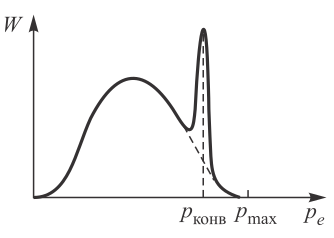
\includegraphics[width = 0.9\textwidth]{Beta-decay spectrum.png}
    \end{center}
    \caption{Форма спектра $\beta$-частиц при разрешенных переходах}
\end{wrapfigure}
где $B = (16\pi^2 / c^4 )D$. В нерелятивистском приближении, которое и имеет место с нашем случае, выражение \eqref{eq: N via E} упрощается, и мы имеем
\begin{equation}\label{eq: N via E simplified}
    \frac{dN}{dE} \approx \sqrt{E}(E_e - E)^2.
\end{equation}
Выражение \eqref{eq: N via E simplified} приводит к спектру, имеющему вид широкого колокола (рис. \hyperref[fig: Beta-decay spectrum]{1}).

Дочерние ядра, возникающие в результате $\beta$-распада, нередко оказываются возбужденными. Возбужденные ядра отдают свою энергию либо излучая $\gamma$-квант, либо передавая избыток энергии одному из электронов с внутренних оболочек атома. Излучаемые в таком процессе электроны имеют строго определенную энергию и называются \textit{конверсионными}.

Конверсия чаще всего происходит на оболочках $K$ или $L$. На спектре, представленном на рис. \hyperref[fig: Beta-decay spectrum]{1}, видна монохроматическая линия, вызванная электронами конверсии. Ширина этой линии в нашем случае является чисто аппаратурной -- по ней можно оценить разрешающую силу спектрометра.

\section{Экспериментальная установка}
Энергию $\beta$-частиц определяют с помощью $\beta$-спектрометров. В работе используется магнитный спектрометр с «короткой линзой». Электроны, испускаемые радиоактивным источником (рис. \hyperref[fig: Beta decay scheme]{2}), попадают в магнитное поле катушки, ось которой параллельна оси $OZ$.

Траектории электронов в магнитном поле представляют собой схематически показанные на рисунке сложные спирали, сходящиеся за катушкой в фокусе, расположенном на оси $OZ$. Силовые линии магнитного поля изображены на рис. \hyperref[fig: Beta decay scheme]{2} тонкими линиями. В фокусе установлен детектор электронов — газоразрядный торцевой счётчик с тонким входным окном, прозрачным для электронов с энергией больше $40$ кэВ, либо сцинтилляционный счетчик. Чувствительным элементом сцинтилляционного счетчика является тонкий кристалл полистирола. При попадании электрона в кристалле возникает световая вспышка -- сцинтилляция, регистрируемая фотоумножителем.
\begin{figure}[H]\label{fig: Beta decay scheme}
    \centering
    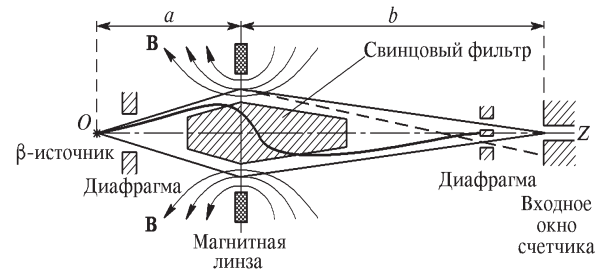
\includegraphics[width = \textwidth]{Beta decay scheme.png}
    \caption{Схема $\beta$-спектрометра с короткой магнитной линзой}
\end{figure}

Для заряженных частиц тонкая катушка эквивалентна линзе. Ее фокусное расстояние $f$ зависит от импульса электронов $p_e$ и от индукции магнитного поля линзы (т. е. от силы тока $I$, протекающего через катушку) следующим образом:
\begin{equation}\label{eq: f via I}
    \frac{1}{f} \propto \frac{I^2}{p_e^2}.
\end{equation}

При заданной силе тока на входное окно счетчика фокусируются электроны с определенным импульсом. Электроны, обладающие другими значениями импульса, при этом не сфокусированы и в основном проходят мимо окна. При изменении тока в катушке на счетчик последовательно фокусируются электроны с разными импульсами. Так как геометрия прибора в течение всего опыта остается неизменной, импульс сфокусированных электронов пропорционален величине тока $I$:
\begin{equation}\label{eq: p_e via I}
    p_e = kI.
\end{equation}

Константа прибора $k$ обычно определяется не из расчета, а из опыта.

Короткая магнитная линза обладает заметной сферической аберрацией, т. е. имеет разные фокусные расстояния для частиц, вылетающих из источника под различными углами. Поэтому приходится устанавливать кольцевые диафрагмы, ограничивающие углы вылета электронов, как это изображено на рис. \hyperref[fig: Beta decay scheme]{2}. Свинцовый фильтр предохраняет счетчик от прямого попадания $\gamma$-лучей, почти всегда сопровождающих $\beta$-распад. Из-за конечных размеров источника, диафрагм и окна счетчика, а также вследствие аберраций при заданной величине фокусного расстояния на счетчик попадают электроны с импульсами, лежащими внутри некоторого интервала от $p_e - \Delta p_e /2$ до $p_e + \Delta p_e /2$. Величина $\Delta p_e$ называется разрешающей способностью $\beta$-спектрометра. Разрешающая способность спектрометра зависит от того, какой угол с осью $OZ$ составляют регистрируемые электроны. Электроны, летящие под небольшим углом к оси спектрометра, практически не отклоняются магнитным полем и попадали бы в окно $\beta$-счетчика при любом токе в линзе, если бы на их пути не было свинцового фильтра. Поэтому разрешение спектрометра зависит не только от размеров кольцевых диафрагм, но и от диаметра свинцового фильтра.

Рассмотрим теперь связь между числом частиц, регистрируемых  установкой, и функцией $W(p_e) = dW/dp_e$ , определяемой формулой \eqref{eq: N via E simplified}.
\begin{equation}\label{eq: N via p_e}
    N(p_e) \approx W(p_e)\Delta p_e,
\end{equation}
где $\Delta p_e$ -- разрешающая способность спектрометра. Формула \eqref{eq: f via I} показывает, что при заданном токе фокусное расстояние магнитной линзы зависит от импульса частиц. Мимо счетчика проходят частицы, для которых фокусное расстояние линзы слишком сильно отличается от нужного, т. е. при недопустимо больших $\Delta f$ . Дифференцируя формулу \eqref{eq: f via I} при постоянном токе, найдем:
\begin{equation}\label{eq: Delta p_e via f}
    \Delta p_e = \frac{1}{2}\frac{\Delta f}{f}p_e.
\end{equation}

Таким образом, ширина интервала $\Delta p_e$ , регистрируемого спектрометром, пропорциональна величине импульса.
Подставив \eqref{eq: Delta p_e via f} в  \eqref{eq: N via p_e} и замечая, что отношение $\Delta f/2f$ определяется геометрией установки и потому постоянно, получим окончательно:
\begin{equation}\label{eq: N via p_e final}
    N(p_e) = CW(p_e)p_e,
\end{equation}
где $C$ -- некоторая константа.

Блок-схема установки для изучения $\beta$-спектров изображена на рис. \hyperref[fig: Exp setup]{3}. Радиоактивный источник ${}^{137}$Cs помещен внутрь откачанной трубы. Электроны, сфокусированные магнитной линзой, попадают в счетчик.
\begin{figure}[H]\label{fig: Exp setup}
    \centering
    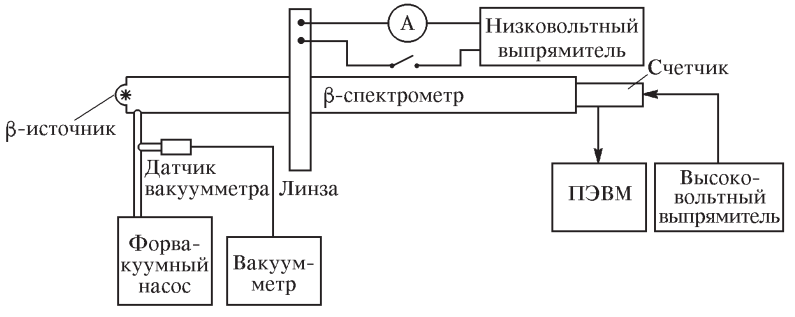
\includegraphics[width = \textwidth]{Exp setup.png}
    \caption{Блок-схема установки для изучения $\beta$-спектра}
\end{figure}
В газоразрядном счетчике они инициируют газовый разряд и тем самым приводят к появлению электрических импульсов на его электродах, которые затем регистрируются пересчетным прибором. В результате попадания электронов в сцинтиллятор на выходе фотоумножителя появляется электрические импульсы, которые заносятся в память персонального компьютера и выводятся на экран монитора. Давление в спектрометре поддерживается на уровне около $0,1$ торр и измеряется термопарным вакуумметром. Лучший вакуум в приборе не нужен, поскольку уже при этом давлении потери энергии электронов малы и их рассеяние незначительно. Откачка осуществляется форвакуумным насосом. Магнитная линза питается постоянным током от выпрямителя. Ток можно повышать до $5$ А, он измеряется цифровым прибором. Высокое напряжение на ФЭУ или газоразрядный счетчик подается от стабилизированного выпрямителя.

\section{Обработка данных}

\subsection{Подготовка установки к работе}
\begin{enumerate}
    \item
    Откачаем воздух из полости спектрометра до давления $P \approx 0,1$ торр. Для этого включим форвакуумный насос и начнём откачку.
    \item 
    Включим вакуумметр и проверим его работу. Для этого установим ток, значение которого указано на установке, $I = 1,5$ A и переведём переключатель в режим измерения давления остаточных газов.
    \item 
    Пока полость спектрометра откачивается, включим ПЭВМ и дождёмся появления на экране титульного листа программы.
    \item 
    Включим формирователь импульсов, питание магнитной линзы и уменьшим ток через нее до нуля.
\end{enumerate}

\subsection{Измерение фона}
\begin{enumerate}
    \item 
    Измерим фоновое излучение, результаты занесём в таблицу.
    \begin{table}[H]\label{tab: N noise result}
        \begin{tabular}{|
            >{\columncolor[HTML]{FFFFFF}}c |
            >{\columncolor[HTML]{FFFFFF}}c |
            >{\columncolor[HTML]{FFFFFF}}c |}
            \hline
            {\color[HTML]{000000} $t$, с} & {\color[HTML]{000000} $N_\text{ф}$, 1/c} & {\color[HTML]{000000} $\varepsilon_{N_\text{ф}}$, $\%$} \\ \hline
            {\color[HTML]{000000} $100$}  & {\color[HTML]{000000} $1,580 \pm 0,126$} & \cellcolor[HTML]{FFFFFF}{\color[HTML]{000000} 7,97}     \\ \hline
        \end{tabular}
        \caption{Измерение фонового излучения}
    \end{table}
    \item 
    Далее за абсолютную погрешность измерения фона будет браться величина \\ $\sigma_{N_\text{ф}} = 0,126\; c^{-1}$.
\end{enumerate}

\subsection{Измерение $\beta$-спектра}
\begin{enumerate}
    \item 
    Постепенно изменяя ток магнитной линзы с шагом $0,2$ А будем проводить измерение $\beta$-спектра. В области конверсионного пика уменьшим шаг до $0,05$ А. Результаты представлены в таблицах ниже.
    \item 
    По результатам измерений постороим график зависимости количества частиц в секунду от силы тока $N(I)$ за вычетом фона.
    \item 
    Зная энергию электронов внутренней конверсии ${}^{137}$Cs, вычислим их импульс, а затем, зная величину силы тока, соответствующей конверсионному пику, $I_{conv} \approx 3,6$А и используя формулу \eqref{eq: p_e via I}, найдём константу прибора $k$ и построим график зависимости $N(T_e)$ в котором аппроксимируем область конверсионного пика гауссианой. При этом полагаем $\sigma_N = \sigma_{N_\text{ф}}$.
    \item 
    Далее построим график зависимости $\frac{\sqrt{N(p)}}{p^{3/2}}(T_e)$ и по нему определим максимальную кинетическую энергию вылетающих электронов по пересечению прямой аппроксимации с осью абсцисс. 
    
    \newpage
    \begin{table}[H]\label{tab: N results part1}
        \centering
        \begin{tabular}{|c|c|c|c|}
            \hline
            \cellcolor[HTML]{FFFFFF}{\color[HTML]{000000} Номер измерения} & \cellcolor[HTML]{FFFFFF}{\color[HTML]{000000} $t$, с} & $I$, А & $N$, 1/с \\ \hline
            \cellcolor[HTML]{FFFFFF}{\color[HTML]{000000} 1} & \cellcolor[HTML]{FFFFFF}{\color[HTML]{000000} 80} & 0,2 & 1,812 \\ \hline
            \cellcolor[HTML]{FFFFFF}{\color[HTML]{000000} 2} & \cellcolor[HTML]{FFFFFF}{\color[HTML]{000000} 80} & 0,4 & 1,862 \\ \hline
            \cellcolor[HTML]{FFFFFF}{\color[HTML]{000000} 3} & \cellcolor[HTML]{FFFFFF}{\color[HTML]{000000} 80} & 0,6 & 1,799 \\ \hline
            \cellcolor[HTML]{FFFFFF}{\color[HTML]{000000} 4} & \cellcolor[HTML]{FFFFFF}{\color[HTML]{000000} 80} & 0,8 & 2,162 \\ \hline
            5                                                & 80                                                & 1,0 & 2,524 \\ \hline
            6                                                & 80                                                & 1,2 & 2,686 \\ \hline
            7                                                & 80                                                & 1,4 & 3,373 \\ \hline
            8                                                & 80                                                & 1,6 & 3,848 \\ \hline
            9                                                & 80                                                & 1,8 & 4,261 \\ \hline
            10                                               & 80                                                & 2,0 & 4,635 \\ \hline
            11                                               & 80                                                & 2,2 & 4,498 \\ \hline
            12                                               & 80                                                & 2,4 & 4,123 \\ \hline
            13                                               & 80                                                & 2,6 & 4,198 \\ \hline
            14                                               & 80                                                & 2,8 & 3,411 \\ \hline
        \end{tabular}
        \caption{Основные измерения часть 1}
        \label{tab: N results part1}
    \end{table}

    \begin{table}[H]\label{tab: N results part2}
        \centering
        \begin{tabular}{|c|
            >{\columncolor[HTML]{FFFFFF}}c |c|c|}
            \hline
            \cellcolor[HTML]{FFFFFF}{\color[HTML]{000000} Номер измерения} & \cellcolor[HTML]{FFFFFF}{\color[HTML]{000000} $t$, с} & $I$, А & $N$, 1/с \\ \hline
            \cellcolor[HTML]{FFFFFF}{\color[HTML]{000000} 15} & \cellcolor[HTML]{FFFFFF}{\color[HTML]{000000} 80} & 3,0  & 2,924 \\ \hline
            \cellcolor[HTML]{FFFFFF}{\color[HTML]{000000} 16} & \cellcolor[HTML]{FFFFFF}{\color[HTML]{000000} 70} & 3,05 & 2,836 \\ \hline
            \cellcolor[HTML]{FFFFFF}{\color[HTML]{000000} 17} & {\color[HTML]{000000} 70}                         & 3,1  & 3,084 \\ \hline
            \cellcolor[HTML]{FFFFFF}{\color[HTML]{000000} 18} & {\color[HTML]{000000} 70}                         & 3,15 & 2,741 \\ \hline
            19                                                & 70                                                & 3,2  & 3,086 \\ \hline
            20                                                & 70                                                & 3,25 & 3,641 \\ \hline
            21                                                & 70                                                & 3,3  & 3,684 \\ \hline
            22                                                & 70                                                & 3,35 & 3,712 \\ \hline
            23                                                & 70                                                & 3,4  & 4,148 \\ \hline
            24                                                & 70                                                & 3,45 & 4,712 \\ \hline
            25                                                & 70                                                & 3,5  & 4,769 \\ \hline
            26                                                & 70                                                & 3,55 & 4,726 \\ \hline
            27                                                & 70                                                & 3,6  & 5,435 \\ \hline
            28                                                & 70                                                & 3,65 & 5,269 \\ \hline
        \end{tabular}
        \caption{Основные измерения часть 2}
    \end{table}

    \begin{table}[H]\label{tab: N results part3}
        \centering
        \begin{tabular}{|c|
            >{\columncolor[HTML]{FFFFFF}}c |c|c|}
            \hline
            \cellcolor[HTML]{FFFFFF}{\color[HTML]{000000} Номер измерения} & \cellcolor[HTML]{FFFFFF}{\color[HTML]{000000} $t$, с} & $I$, А & $N$, 1/с \\ \hline
            \cellcolor[HTML]{FFFFFF}{\color[HTML]{000000} 29} & \cellcolor[HTML]{FFFFFF}{\color[HTML]{000000} 70} & 3,7  & 4,897 \\ \hline
            \cellcolor[HTML]{FFFFFF}{\color[HTML]{000000} 30} & \cellcolor[HTML]{FFFFFF}{\color[HTML]{000000} 70} & 3,75 & 5,169 \\ \hline
            \cellcolor[HTML]{FFFFFF}{\color[HTML]{000000} 31} & {\color[HTML]{000000} 70}                         & 3,8  & 4,273 \\ \hline
            \cellcolor[HTML]{FFFFFF}{\color[HTML]{000000} 32} & {\color[HTML]{000000} 70}                         & 3,85 & 3,955 \\ \hline
            33                                                & 70                                                & 3,9  & 3,156 \\ \hline
            34                                                & 70                                                & 3,95 & 2,827 \\ \hline
            35                                                & 80                                                & 4,0  & 2,336 \\ \hline
        \end{tabular}
        \caption{Основные измерения часть 3}
    \end{table}
    
\end{enumerate}

\section{Вывод}
В данной работе проводилось исследование энергнетического спектра $\beta$-частиц при помощи магнитного спектрометра. В результате удалось:
\begin{itemize}
    \item
    снять зависимость количества вылетающих в единицу времени $\beta$-частиц распада от их энергии
    \item 
    выделить в спектре теоретически предсказанный конверсионный пик
    \item 
    построить по полученным данным график Ферми и, экстраполировав аппроксимирующую прямую, вычислить максимальную энергию вылетающих электронов
\end{itemize}

\newpage
%%%%%%%%%%%%%%%%%%%%%%%%% Графики

\begin{figure}[H]\label{fig: N(I)}
    \centering
    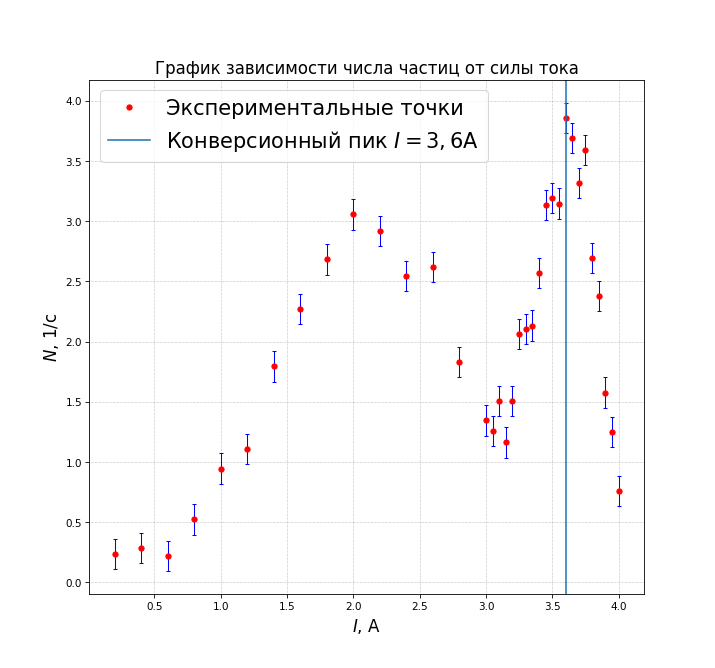
\includegraphics[width = 0.65\textwidth]{N(I).png}
\end{figure}

\begin{figure}[H]\label{fig: N(T)}
    \centering
    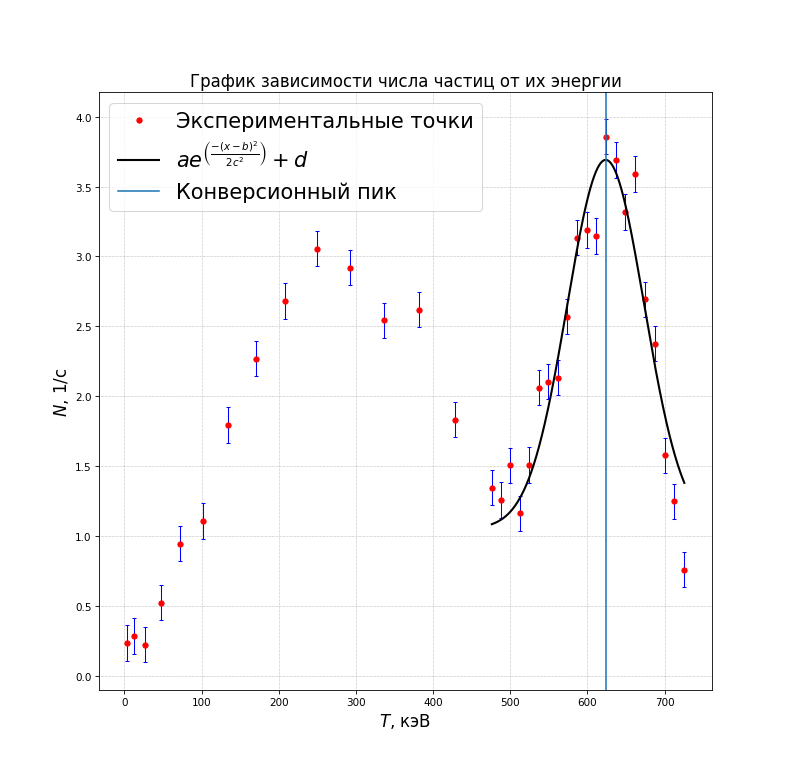
\includegraphics[width = 0.65\textwidth]{N(T).png}
\end{figure}
$$
    a = 2.64,\; b = 623,74,\; c = 49,9,\; d = 1,05.
$$

\newpage
\begin{figure}[H]\label{fig: sqrtN_p32(T)}
    \centering
    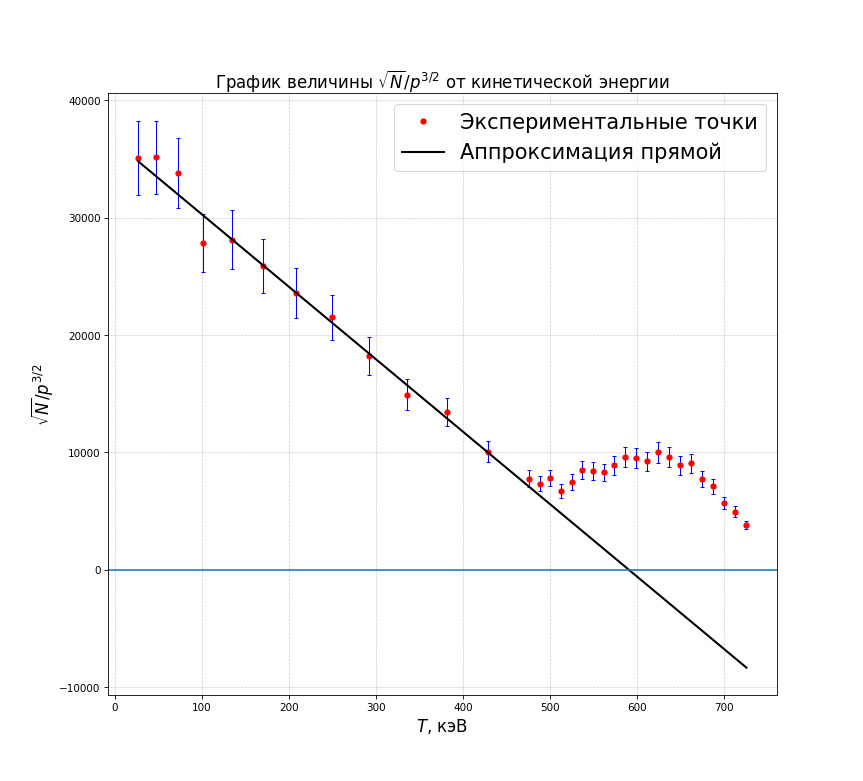
\includegraphics[width = 1\textwidth]{sqrtN_p32(T).png}
\end{figure}
При построении графика не были учтены первые две точки из-за слишком большого значения величины $\sqrt{N}/p^{3/2}$ и её погрешности.
$$
    \sigma_{f(T)} = \frac{1}{\sqrt{2N}}\frac{\sigma_N}{p^{3/2}} 
$$
$$
    k = (-61,8 \pm 1,45);\; b = (36472,9 \pm 600);\; \Rightarrow \fbox{T_{max} = (590,2 \pm 16,9)\text{ кэВ}} 
$$

%%%%%%%%%%%%%%%%%%%%%%%%%
\end{document}
